\section{Results}\label{sec:results}

\subsection{Functional: xfstests}\label{sec:xfstests}

\Cref{tab:xfs} counts the \xfsTotal{} tests by what check said of each,
read from check's own output for every test. Both sweeps ran on commit
\texttt{\commitBeamfs}, with a budget of 14\,400\,s per test. On x86-64
\xfsXRan{} tests ran and all passed, generic/476, a long multi-process
stress test, in \xfsXfullSeconds\,s. On aarch64 \xfsARan{} ran and
\xfsAPass{} passed; the failure is generic/476, which the harness stopped
at its budget after \xfsAfullSeconds\,s, before check gave a verdict. Run
alone on the same node and image with a longer budget, it passed, in
\xfsAsoloSeconds\,s (\texttt{\sweepAsoloName}).

The other tests did not run: check declined them. On x86-64,
\xfsXNrFeature{} were declined because \bfs does not implement what they
test, \xfsXNrEnv{} because the test image or the virtual machine lacks
what they need, and \xfsXNrScope{} because they apply to other
filesystems only; on aarch64, \xfsANrFeature, \xfsANrEnv{} and
\xfsANrScope. Only \xfsNotrunDifferList{} ran on one architecture and not the
other: it passed on aarch64, and on x86-64 check declined it for want
of procfs \texttt{uid\_map} support. A declined test is untested, not passed: reflinks,
quotas, \texttt{O\_DIRECT}, fallocate modes other than allocation,
encryption, extended attributes and ACLs, among others, are outside what
this suite says about \bfs, and the environment's share (device-mapper
targets, absent tools) is a gap of the test bed, not of \bfs.

These counts are not the ones the harness first printed. Before version
2.4.0 it recorded a declined test as passed, because check counts it in
its ``Passed all'' line, and the aarch64 sweep was saved as 733 passes
and one failure. The aarch64 counts here are recomputed from the output
of check that the harness kept for each test; the x86-64 sweep was run
again under 2.5.1, which records a declined test as such, its budget and
every recovery of the node (\cref{sec:selfaudit}). Two earlier x86-64
sweeps of the same commit are superseded: one saved as 734 passes, whose
per-test output was overwritten by the sweeps that followed, and one
stopped after \xfsSupDone{} tests once its budget, the default
1\,900\,s, had stopped generic/476.

\begin{table}[t]
\centering
\caption{xfstests auto group, \xfsTotal{} tests, by what check said of
each test. Declined tests by the reason check gave; groups of fewer
than four tests are summed per kind, all \xfsGroups{} are in the
derived file xfstests.csv.}
\label{tab:xfs}
\footnotesize
\begin{tabular}{@{}llrr@{}}
\toprule
 & & x86-64 & aarch64 \\
\midrule
passed & & 122 & 122 \\
failed & & 0 & 1 \\
declined by check & & 612 & 611 \\
\midrule
\multicolumn{4}{@{}l}{declined for} \\
\quad reflink & feature & 172 & 172 \\
\quad fallocate modes & feature & 66 & 66 \\
\quad O\_DIRECT & feature & 50 & 50 \\
\quad quotas & feature & 30 & 30 \\
\quad shutdown ioctl & feature & 29 & 29 \\
\quad encryption & feature & 26 & 26 \\
\quad extended attributes & feature & 22 & 22 \\
\quad exchange-range & feature & 19 & 19 \\
\quad deduplication & feature & 14 & 14 \\
\quad ACLs & feature & 13 & 13 \\
\quad inode flags & feature & 12 & 12 \\
\quad swap files & feature & 12 & 12 \\
\quad device nodes, FIFOs & feature & 8 & 8 \\
\quad idmapped mounts & feature & 6 & 6 \\
\quad freeze & feature & 5 & 5 \\
\quad O\_TMPFILE & feature & 4 & 4 \\
\quad renameat2 flags & feature & 4 & 4 \\
\quad 13 other features & feature & 19 & 19 \\
\addlinespace[2pt]
\quad device-mapper target & environment & 48 & 48 \\
\quad tool absent from the image & environment & 16 & 16 \\
\quad richacl & environment & 9 & 9 \\
\quad device size & environment & 7 & 7 \\
\quad DAX & environment & 5 & 5 \\
\quad log device & environment & 4 & 4 \\
\quad scsi\_debug & environment & 4 & 4 \\
\quad 4 other needs & environment & 5 & 4 \\
\addlinespace[2pt]
\quad other filesystems only & scope & 3 & 3 \\
\bottomrule
\end{tabular}

\end{table}

\subsection{Filesystem comparison}\label{sec:multifs}

\Cref{fig:multifs} shows run 4 and \cref{tab:multifs} all three runs.
\bfs returned the correct file in every attack that received flips, up
to \mfBeamfsMaxFlips{} flips during one read, in all three runs. At
$10^{6}$\,ppm, ext4 returned wrong data with a successful read after
\mfExtFourFlipsMax{} flip, ext3 after \mfExtThreeFlipsMin{} to
\mfExtThreeFlipsMax{}, in every run: silent corruption. btrfs, after
\mfBtrfsFlipsMin{} flips, refused the read on a checksum mismatch.
squashfs was never exercised: the bench builds its image offline and
gave the injector no target.

The doses differ by design and are reported as received, not equalised.
emufi draws once per hook and per bio, and a filesystem receives flips
in proportion to the bios its read issues: one for ext4, about two per
data block for \bfs (\cref{sec:readpath}), which is why the other
filesystems received no flip at $10^{3}$ and $10^{5}$\,ppm. What the
comparison measures is the outcome per flip received: \bfs absorbed two
orders of magnitude more flips than any other filesystem and returned
the right bytes; ext4 and ext3 returned wrong bytes without an error;
btrfs detected and refused. It is not a ranking of these filesystems in
general.

After every attack the volume was remounted with the injector off and
all twelve files of every filesystem hashed intact, including those of
ext4 and ext3 after their silent corruption: the wrong bytes were made
in the read path, not on the medium.

\begin{figure}[t]
\centering
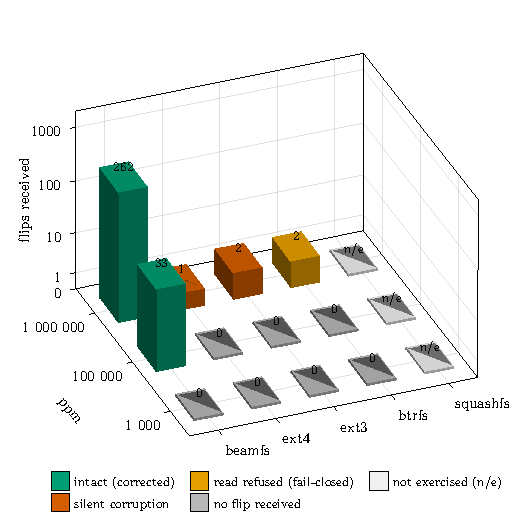
\includegraphics[width=\columnwidth]{figures/multifs-3d.pdf}
\caption{Filesystem comparison, run 4: flips received during one read
of the target file (logarithmic, number on each bar) and outcome, for
each injection probability per hook call (ppm).}
\label{fig:multifs}
\end{figure}

\begin{table}[t]
\centering
\caption{Filesystem comparison, three runs: flips received and outcome
(I intact, S silent corruption, R read refused, N no flip,
n/e not exercised).}
\label{tab:multifs}
\footnotesize
\begin{tabular}{@{}llccc@{}}
\toprule
FS & ppm & run 2 & run 3 & run 4 \\
\midrule
beamfs & 1\,000 & 0\,N & 0\,N & 0\,N \\
 & 100\,000 & 20\,I & 22\,I & 33\,I \\
 & 1\,000\,000 & 265\,I & 265\,I & 262\,I \\
\addlinespace[2pt]
ext4 & 1\,000 & 0\,N & 0\,N & 0\,N \\
 & 100\,000 & 0\,N & 0\,N & 0\,N \\
 & 1\,000\,000 & 1\,S & 1\,S & 1\,S \\
\addlinespace[2pt]
ext3 & 1\,000 & 0\,N & 0\,N & 0\,N \\
 & 100\,000 & 0\,N & 0\,N & 0\,N \\
 & 1\,000\,000 & 3\,S & 2\,S & 2\,S \\
\addlinespace[2pt]
btrfs & 1\,000 & 0\,N & 0\,N & 0\,N \\
 & 100\,000 & 0\,N & 0\,N & 0\,N \\
 & 1\,000\,000 & 2\,R & 2\,R & 2\,R \\
\addlinespace[2pt]
squashfs & 1\,000 & n/e & n/e & n/e \\
 & 100\,000 & n/e & n/e & n/e \\
 & 1\,000\,000 & n/e & n/e & n/e \\
\bottomrule
\end{tabular}

\end{table}

\subsection{Cluster}\label{sec:cluster}

In run 4 all twelve cases were exercised (\cref{fig:cluster},
\cref{tab:cluster}): \clRunFourIntact{} returned the correct file after
flips, \clRunFourNoFlip{} received none at $10^{3}$\,ppm. In run 3,
\texttt{compute01} was not exercised, and \texttt{beamfs-master} at
$10^{6}$\,ppm refused the read after \clRunThreeRefusedFlips{} flips
(\cref{sec:indirect}). In run 2 no cluster case was exercised.

\begin{figure*}[t]
\centering
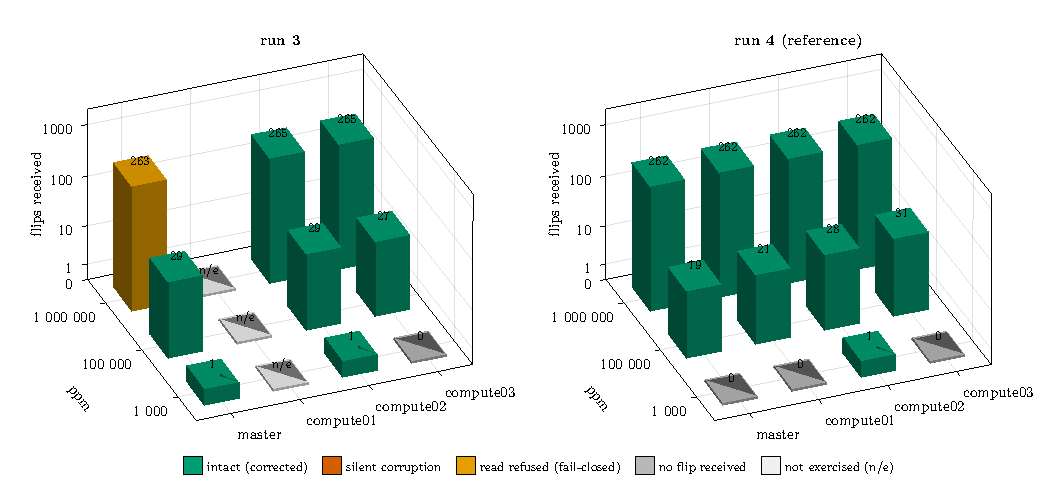
\includegraphics[width=\textwidth]{figures/cluster-3d.pdf}
\caption{Cluster campaign, runs 3 and 4: flips received by each node's
attack and outcome, for each injection probability per hook call (ppm).}
\label{fig:cluster}
\end{figure*}

\begin{table}[t]
\centering
\caption{Cluster campaign: flips received and outcome (codes as in
\cref{tab:multifs}). Run 2 exercised no case.}
\label{tab:cluster}
\footnotesize
\begin{tabular}{@{}llcc@{}}
\toprule
node & ppm & run 3 & run 4 \\
\midrule
master & 1\,000 & 1\,I & 0\,N \\
 & 100\,000 & 29\,I & 19\,I \\
 & 1\,000\,000 & 263\,R & 262\,I \\
\addlinespace[2pt]
compute01 & 1\,000 & n/e & 0\,N \\
 & 100\,000 & n/e & 21\,I \\
 & 1\,000\,000 & n/e & 262\,I \\
\addlinespace[2pt]
compute02 & 1\,000 & 1\,I & 1\,I \\
 & 100\,000 & 29\,I & 28\,I \\
 & 1\,000\,000 & 265\,I & 262\,I \\
\addlinespace[2pt]
compute03 & 1\,000 & 0\,N & 0\,N \\
 & 100\,000 & 27\,I & 31\,I \\
 & 1\,000\,000 & 265\,I & 262\,I \\
\bottomrule
\end{tabular}

\end{table}

\subsection{Indirect blocks}\label{sec:indirect}

In run 3 the cluster filter was the interval spanning the file, which
contains its indirect block. On \texttt{beamfs-master} at
$10^{6}$\,ppm the kernel logged four times
\begin{lstlisting}
beamfs/inline: corrupted indirect pointer ino=11 iblock=45
  slot=33 phys=18014398509500044 (out of [17502, 262144))
\end{lstlisting}
\noindent That value is
$2^{54}+18\,060$: bit 54 of the pointer in slot 33 was flipped in the
read buffer, the true pointer being 18\,060. On this code path the
Reed-Solomon verify decodes a copy of the freshly read indirect block,
finds a correctable error and lets the lookup proceed
(\cref{sec:indirect-design}); the lookup read the pointer from the
buffer, found it outside the data area and failed. The read was refused,
no wrong byte was returned, and the twelve files verified intact
afterwards.

In the filesystem comparison the reconstruction of
\cref{sec:injector} attributes \indHits{} flips to the target file's
indirect block, at slots \indSlots{}, including one in run 4 through the
second hook. The file uses 57 pointers (69 data blocks, 12 of them
direct), slots 0 to 56: none of these flips touched a pointer in use,
and the reads were unaffected.

These events show the fail-closed contract holding for a pointer flipped
out of range. They do not test the residual of
\cref{sec:indirect-design}: a flip that keeps a pointer inside the data
area and on an allocated block would, on these volumes, return another
block's bytes.
